\documentclass[12pt]{article} 
% \documentclass[12pt]{amsart} 

% Custom definitions
% To use this customization file, insert the line "% Custom definitions
% To use this customization file, insert the line "% Custom definitions
% To use this customization file, insert the line "\input{custom}" in the header of the tex file.

% Formatting

\tolerance=1000
\usepackage[margin=1in]{geometry}


% Packages

% \usepackage{amssymb,latexsym}
\usepackage{amssymb,amsfonts,amsmath,latexsym,amsthm}
\usepackage[usenames,dvipsnames]{color}
\usepackage[]{graphicx}
\usepackage[space]{grffile}
\usepackage{mathrsfs}   % fancy math font
% \usepackage[font=small,skip=0pt]{caption}
\usepackage[skip=0pt]{caption}
\usepackage{subcaption}
\usepackage{verbatim}
\usepackage{url}
\usepackage{bm}
\usepackage{dsfont}
\usepackage{extarrows}
\usepackage{multirow}
% \usepackage{wrapfig}
% \usepackage{epstopdf}
\usepackage{rotating}
\usepackage{tikz}
\usetikzlibrary{fit}					% fitting shapes to coordinates
%\usetikzlibrary{backgrounds}	% drawing the background after the foreground

\usepackage{fancyhdr}

\fancypagestyle{firststyle}{
   \fancyhf{}
   \renewcommand{\footrulewidth}{0.4pt}
   \fancyfoot[L]{\footnotesize This work is licensed under a \href{http://creativecommons.org/licenses/by-nc-nd/4.0/}{Creative Commons BY-NC-ND 4.0 International License}.\\ Jeffrey W. Miller (2015). \textit{Lecture Notes on Bayesian Statistics}. Duke University, Durham, NC.}
}


% \usepackage[dvipdfm,colorlinks,citecolor=blue,linkcolor=blue,urlcolor=blue]{hyperref}
\usepackage[colorlinks,citecolor=blue,linkcolor=blue,urlcolor=blue]{hyperref}
%\usepackage{hyperref}
\usepackage[authoryear,round]{natbib}


%  Theorems, etc.

\theoremstyle{plain}
\newtheorem{theorem}{Theorem}[section]
\newtheorem{corollary}[theorem]{Corollary}
\newtheorem{lemma}[theorem]{Lemma}
\newtheorem{proposition}[theorem]{Proposition}
\newtheorem{condition}[theorem]{Condition}
% \newtheorem{conditions}[theorem]{Conditions}

\theoremstyle{definition}
\newtheorem{definition}[theorem]{Definition}
% \newtheorem*{unnumbered-definition}{Definition}
\newtheorem{example}[theorem]{Example}
\theoremstyle{remark}
\newtheorem*{remark}{Remark}
\numberwithin{equation}{section}



% Document-specific shortcuts
\newcommand{\btheta}{{\bm\theta}}
\newcommand{\bbtheta}{{\pmb{\bm\theta}}}

\newcommand{\commentary}[1]{\ifx\showcommentary\undefined\else \emph{#1}\fi}

\newcommand{\term}[1]{\textit{\textbf{#1}}}

% Math shortcuts

% Probability distributions
\DeclareMathOperator*{\Exp}{Exp}
\DeclareMathOperator*{\TExp}{TExp}
\DeclareMathOperator*{\Bernoulli}{Bernoulli}
\DeclareMathOperator*{\Beta}{Beta}
\DeclareMathOperator*{\Ga}{Gamma}
\DeclareMathOperator*{\TGamma}{TGamma}
\DeclareMathOperator*{\Poisson}{Poisson}
\DeclareMathOperator*{\Binomial}{Binomial}
\DeclareMathOperator*{\NormalGamma}{NormalGamma}
\DeclareMathOperator*{\InvGamma}{InvGamma}
\DeclareMathOperator*{\Cauchy}{Cauchy}
\DeclareMathOperator*{\Uniform}{Uniform}
\DeclareMathOperator*{\Gumbel}{Gumbel}
\DeclareMathOperator*{\Pareto}{Pareto}
\DeclareMathOperator*{\Mono}{Mono}
\DeclareMathOperator*{\Geometric}{Geometric}
\DeclareMathOperator*{\Wishart}{Wishart}

% Math operators
\DeclareMathOperator*{\argmin}{arg\,min}
\DeclareMathOperator*{\argmax}{arg\,max}
\DeclareMathOperator*{\Cov}{Cov}
\DeclareMathOperator*{\diag}{diag}
\DeclareMathOperator*{\median}{median}
\DeclareMathOperator*{\Vol}{Vol}

% Math characters
\newcommand{\R}{\mathbb{R}}
\newcommand{\Z}{\mathbb{Z}}
\newcommand{\E}{\mathbb{E}}
\renewcommand{\Pr}{\mathbb{P}}
\newcommand{\I}{\mathds{1}}
\newcommand{\V}{\mathbb{V}}

\newcommand{\A}{\mathcal{A}}
\newcommand{\C}{\mathcal{C}}
\newcommand{\D}{\mathcal{D}}
\newcommand{\Hcal}{\mathcal{H}}
\newcommand{\M}{\mathcal{M}}
\newcommand{\N}{\mathcal{N}}
\newcommand{\X}{\mathcal{X}}
\newcommand{\Zcal}{\mathcal{Z}}
\renewcommand{\P}{\mathcal{P}}

\newcommand{\T}{\mathtt{T}}
\renewcommand{\emptyset}{\varnothing}


% Miscellaneous commands
\newcommand{\iid}{\stackrel{\mathrm{iid}}{\sim}}
\newcommand{\matrixsmall}[1]{\bigl(\begin{smallmatrix}#1\end{smallmatrix} \bigr)}

\newcommand{\items}[1]{\begin{itemize} #1 \end{itemize}}

\newcommand{\todo}[1]{\emph{\textcolor{red}{(#1)}}}

\newcommand{\branch}[4]{
\left\{
	\begin{array}{ll}
		#1  & \mbox{if } #2 \\
		#3 & \mbox{if } #4
	\end{array}
\right.
}

% approximately proportional to
\def\app#1#2{%
  \mathrel{%
    \setbox0=\hbox{$#1\sim$}%
    \setbox2=\hbox{%
      \rlap{\hbox{$#1\propto$}}%
      \lower1.3\ht0\box0%
    }%
    \raise0.25\ht2\box2%
  }%
}
\def\approxprop{\mathpalette\app\relax}

% \newcommand{\approptoinn}[2]{\mathrel{\vcenter{
  % \offinterlineskip\halign{\hfil$##$\cr
    % #1\propto\cr\noalign{\kern2pt}#1\sim\cr\noalign{\kern-2pt}}}}}

% \newcommand{\approxpropto}{\mathpalette\approptoinn\relax}





" in the header of the tex file.

% Formatting

\tolerance=1000
\usepackage[margin=1in]{geometry}


% Packages

% \usepackage{amssymb,latexsym}
\usepackage{amssymb,amsfonts,amsmath,latexsym,amsthm}
\usepackage[usenames,dvipsnames]{color}
\usepackage[]{graphicx}
\usepackage[space]{grffile}
\usepackage{mathrsfs}   % fancy math font
% \usepackage[font=small,skip=0pt]{caption}
\usepackage[skip=0pt]{caption}
\usepackage{subcaption}
\usepackage{verbatim}
\usepackage{url}
\usepackage{bm}
\usepackage{dsfont}
\usepackage{extarrows}
\usepackage{multirow}
% \usepackage{wrapfig}
% \usepackage{epstopdf}
\usepackage{rotating}
\usepackage{tikz}
\usetikzlibrary{fit}					% fitting shapes to coordinates
%\usetikzlibrary{backgrounds}	% drawing the background after the foreground

\usepackage{fancyhdr}

\fancypagestyle{firststyle}{
   \fancyhf{}
   \renewcommand{\footrulewidth}{0.4pt}
   \fancyfoot[L]{\footnotesize This work is licensed under a \href{http://creativecommons.org/licenses/by-nc-nd/4.0/}{Creative Commons BY-NC-ND 4.0 International License}.\\ Jeffrey W. Miller (2015). \textit{Lecture Notes on Bayesian Statistics}. Duke University, Durham, NC.}
}


% \usepackage[dvipdfm,colorlinks,citecolor=blue,linkcolor=blue,urlcolor=blue]{hyperref}
\usepackage[colorlinks,citecolor=blue,linkcolor=blue,urlcolor=blue]{hyperref}
%\usepackage{hyperref}
\usepackage[authoryear,round]{natbib}


%  Theorems, etc.

\theoremstyle{plain}
\newtheorem{theorem}{Theorem}[section]
\newtheorem{corollary}[theorem]{Corollary}
\newtheorem{lemma}[theorem]{Lemma}
\newtheorem{proposition}[theorem]{Proposition}
\newtheorem{condition}[theorem]{Condition}
% \newtheorem{conditions}[theorem]{Conditions}

\theoremstyle{definition}
\newtheorem{definition}[theorem]{Definition}
% \newtheorem*{unnumbered-definition}{Definition}
\newtheorem{example}[theorem]{Example}
\theoremstyle{remark}
\newtheorem*{remark}{Remark}
\numberwithin{equation}{section}



% Document-specific shortcuts
\newcommand{\btheta}{{\bm\theta}}
\newcommand{\bbtheta}{{\pmb{\bm\theta}}}

\newcommand{\commentary}[1]{\ifx\showcommentary\undefined\else \emph{#1}\fi}

\newcommand{\term}[1]{\textit{\textbf{#1}}}

% Math shortcuts

% Probability distributions
\DeclareMathOperator*{\Exp}{Exp}
\DeclareMathOperator*{\TExp}{TExp}
\DeclareMathOperator*{\Bernoulli}{Bernoulli}
\DeclareMathOperator*{\Beta}{Beta}
\DeclareMathOperator*{\Ga}{Gamma}
\DeclareMathOperator*{\TGamma}{TGamma}
\DeclareMathOperator*{\Poisson}{Poisson}
\DeclareMathOperator*{\Binomial}{Binomial}
\DeclareMathOperator*{\NormalGamma}{NormalGamma}
\DeclareMathOperator*{\InvGamma}{InvGamma}
\DeclareMathOperator*{\Cauchy}{Cauchy}
\DeclareMathOperator*{\Uniform}{Uniform}
\DeclareMathOperator*{\Gumbel}{Gumbel}
\DeclareMathOperator*{\Pareto}{Pareto}
\DeclareMathOperator*{\Mono}{Mono}
\DeclareMathOperator*{\Geometric}{Geometric}
\DeclareMathOperator*{\Wishart}{Wishart}

% Math operators
\DeclareMathOperator*{\argmin}{arg\,min}
\DeclareMathOperator*{\argmax}{arg\,max}
\DeclareMathOperator*{\Cov}{Cov}
\DeclareMathOperator*{\diag}{diag}
\DeclareMathOperator*{\median}{median}
\DeclareMathOperator*{\Vol}{Vol}

% Math characters
\newcommand{\R}{\mathbb{R}}
\newcommand{\Z}{\mathbb{Z}}
\newcommand{\E}{\mathbb{E}}
\renewcommand{\Pr}{\mathbb{P}}
\newcommand{\I}{\mathds{1}}
\newcommand{\V}{\mathbb{V}}

\newcommand{\A}{\mathcal{A}}
\newcommand{\C}{\mathcal{C}}
\newcommand{\D}{\mathcal{D}}
\newcommand{\Hcal}{\mathcal{H}}
\newcommand{\M}{\mathcal{M}}
\newcommand{\N}{\mathcal{N}}
\newcommand{\X}{\mathcal{X}}
\newcommand{\Zcal}{\mathcal{Z}}
\renewcommand{\P}{\mathcal{P}}

\newcommand{\T}{\mathtt{T}}
\renewcommand{\emptyset}{\varnothing}


% Miscellaneous commands
\newcommand{\iid}{\stackrel{\mathrm{iid}}{\sim}}
\newcommand{\matrixsmall}[1]{\bigl(\begin{smallmatrix}#1\end{smallmatrix} \bigr)}

\newcommand{\items}[1]{\begin{itemize} #1 \end{itemize}}

\newcommand{\todo}[1]{\emph{\textcolor{red}{(#1)}}}

\newcommand{\branch}[4]{
\left\{
	\begin{array}{ll}
		#1  & \mbox{if } #2 \\
		#3 & \mbox{if } #4
	\end{array}
\right.
}

% approximately proportional to
\def\app#1#2{%
  \mathrel{%
    \setbox0=\hbox{$#1\sim$}%
    \setbox2=\hbox{%
      \rlap{\hbox{$#1\propto$}}%
      \lower1.3\ht0\box0%
    }%
    \raise0.25\ht2\box2%
  }%
}
\def\approxprop{\mathpalette\app\relax}

% \newcommand{\approptoinn}[2]{\mathrel{\vcenter{
  % \offinterlineskip\halign{\hfil$##$\cr
    % #1\propto\cr\noalign{\kern2pt}#1\sim\cr\noalign{\kern-2pt}}}}}

% \newcommand{\approxpropto}{\mathpalette\approptoinn\relax}





" in the header of the tex file.

% Formatting

\tolerance=1000
\usepackage[margin=1in]{geometry}


% Packages

% \usepackage{amssymb,latexsym}
\usepackage{amssymb,amsfonts,amsmath,latexsym,amsthm}
\usepackage[usenames,dvipsnames]{color}
\usepackage[]{graphicx}
\usepackage[space]{grffile}
\usepackage{mathrsfs}   % fancy math font
% \usepackage[font=small,skip=0pt]{caption}
\usepackage[skip=0pt]{caption}
\usepackage{subcaption}
\usepackage{verbatim}
\usepackage{url}
\usepackage{bm}
\usepackage{dsfont}
\usepackage{extarrows}
\usepackage{multirow}
% \usepackage{wrapfig}
% \usepackage{epstopdf}
\usepackage{rotating}
\usepackage{tikz}
\usetikzlibrary{fit}					% fitting shapes to coordinates
%\usetikzlibrary{backgrounds}	% drawing the background after the foreground

\usepackage{fancyhdr}

\fancypagestyle{firststyle}{
   \fancyhf{}
   \renewcommand{\footrulewidth}{0.4pt}
   \fancyfoot[L]{\footnotesize This work is licensed under a \href{http://creativecommons.org/licenses/by-nc-nd/4.0/}{Creative Commons BY-NC-ND 4.0 International License}.\\ Jeffrey W. Miller (2015). \textit{Lecture Notes on Bayesian Statistics}. Duke University, Durham, NC.}
}


% \usepackage[dvipdfm,colorlinks,citecolor=blue,linkcolor=blue,urlcolor=blue]{hyperref}
\usepackage[colorlinks,citecolor=blue,linkcolor=blue,urlcolor=blue]{hyperref}
%\usepackage{hyperref}
\usepackage[authoryear,round]{natbib}


%  Theorems, etc.

\theoremstyle{plain}
\newtheorem{theorem}{Theorem}[section]
\newtheorem{corollary}[theorem]{Corollary}
\newtheorem{lemma}[theorem]{Lemma}
\newtheorem{proposition}[theorem]{Proposition}
\newtheorem{condition}[theorem]{Condition}
% \newtheorem{conditions}[theorem]{Conditions}

\theoremstyle{definition}
\newtheorem{definition}[theorem]{Definition}
% \newtheorem*{unnumbered-definition}{Definition}
\newtheorem{example}[theorem]{Example}
\theoremstyle{remark}
\newtheorem*{remark}{Remark}
\numberwithin{equation}{section}



% Document-specific shortcuts
\newcommand{\btheta}{{\bm\theta}}
\newcommand{\bbtheta}{{\pmb{\bm\theta}}}

\newcommand{\commentary}[1]{\ifx\showcommentary\undefined\else \emph{#1}\fi}

\newcommand{\term}[1]{\textit{\textbf{#1}}}

% Math shortcuts

% Probability distributions
\DeclareMathOperator*{\Exp}{Exp}
\DeclareMathOperator*{\TExp}{TExp}
\DeclareMathOperator*{\Bernoulli}{Bernoulli}
\DeclareMathOperator*{\Beta}{Beta}
\DeclareMathOperator*{\Ga}{Gamma}
\DeclareMathOperator*{\TGamma}{TGamma}
\DeclareMathOperator*{\Poisson}{Poisson}
\DeclareMathOperator*{\Binomial}{Binomial}
\DeclareMathOperator*{\NormalGamma}{NormalGamma}
\DeclareMathOperator*{\InvGamma}{InvGamma}
\DeclareMathOperator*{\Cauchy}{Cauchy}
\DeclareMathOperator*{\Uniform}{Uniform}
\DeclareMathOperator*{\Gumbel}{Gumbel}
\DeclareMathOperator*{\Pareto}{Pareto}
\DeclareMathOperator*{\Mono}{Mono}
\DeclareMathOperator*{\Geometric}{Geometric}
\DeclareMathOperator*{\Wishart}{Wishart}

% Math operators
\DeclareMathOperator*{\argmin}{arg\,min}
\DeclareMathOperator*{\argmax}{arg\,max}
\DeclareMathOperator*{\Cov}{Cov}
\DeclareMathOperator*{\diag}{diag}
\DeclareMathOperator*{\median}{median}
\DeclareMathOperator*{\Vol}{Vol}

% Math characters
\newcommand{\R}{\mathbb{R}}
\newcommand{\Z}{\mathbb{Z}}
\newcommand{\E}{\mathbb{E}}
\renewcommand{\Pr}{\mathbb{P}}
\newcommand{\I}{\mathds{1}}
\newcommand{\V}{\mathbb{V}}

\newcommand{\A}{\mathcal{A}}
\newcommand{\C}{\mathcal{C}}
\newcommand{\D}{\mathcal{D}}
\newcommand{\Hcal}{\mathcal{H}}
\newcommand{\M}{\mathcal{M}}
\newcommand{\N}{\mathcal{N}}
\newcommand{\X}{\mathcal{X}}
\newcommand{\Zcal}{\mathcal{Z}}
\renewcommand{\P}{\mathcal{P}}

\newcommand{\T}{\mathtt{T}}
\renewcommand{\emptyset}{\varnothing}


% Miscellaneous commands
\newcommand{\iid}{\stackrel{\mathrm{iid}}{\sim}}
\newcommand{\matrixsmall}[1]{\bigl(\begin{smallmatrix}#1\end{smallmatrix} \bigr)}

\newcommand{\items}[1]{\begin{itemize} #1 \end{itemize}}

\newcommand{\todo}[1]{\emph{\textcolor{red}{(#1)}}}

\newcommand{\branch}[4]{
\left\{
	\begin{array}{ll}
		#1  & \mbox{if } #2 \\
		#3 & \mbox{if } #4
	\end{array}
\right.
}

% approximately proportional to
\def\app#1#2{%
  \mathrel{%
    \setbox0=\hbox{$#1\sim$}%
    \setbox2=\hbox{%
      \rlap{\hbox{$#1\propto$}}%
      \lower1.3\ht0\box0%
    }%
    \raise0.25\ht2\box2%
  }%
}
\def\approxprop{\mathpalette\app\relax}

% \newcommand{\approptoinn}[2]{\mathrel{\vcenter{
  % \offinterlineskip\halign{\hfil$##$\cr
    % #1\propto\cr\noalign{\kern2pt}#1\sim\cr\noalign{\kern-2pt}}}}}

% \newcommand{\approxpropto}{\mathpalette\approptoinn\relax}






\setcounter{tocdepth}{1}

\graphicspath{{figures/}}

\title{Chapter 4: Univariate Normal Model}
\author{}
\date{}

\def\showcommentary{1}

\begin{document}
\maketitle

\tableofcontents 

\thispagestyle{firststyle}

\vspace{5em}

\section{The normal distribution}

The normal distribution $\N(\mu,\sigma^2)$ (sometimes called the Gaussian distribution) with mean $\mu\in\R$ and variance $\sigma^2 > 0$ (standard deviation $\sigma =\sqrt{\sigma^2}$) has p.d.f.
$$\N(x\mid\mu,\sigma^2) =\frac{1}{\sqrt{2\pi\sigma^2}}\exp\Big(-\frac{1}{2\sigma^2}(x-\mu)^2\Big) $$
for $x\in\R$. In Bayesian calculations, it is often more convenient to write the p.d.f.\ in terms of the precision, or inverse variance, $\lambda = 1/\sigma^2$ rather than the variance. In this parametrization, the p.d.f.\ is
$$\N(x\mid\mu,\lambda^{-1}) =\sqrt{\frac{\lambda}{2\pi}}\exp\big(-\tfrac{1}{2}\lambda (x-\mu)^2\big) $$
since $\sigma^2 = 1/\lambda =\lambda^{-1}$.
%(Warning: Some authors write $\N(\mu,\sigma)$ instead of $\N(\mu,\sigma^2)$, so be careful to know what parametrization is being used.)

\begin{figure}
  \begin{center}
    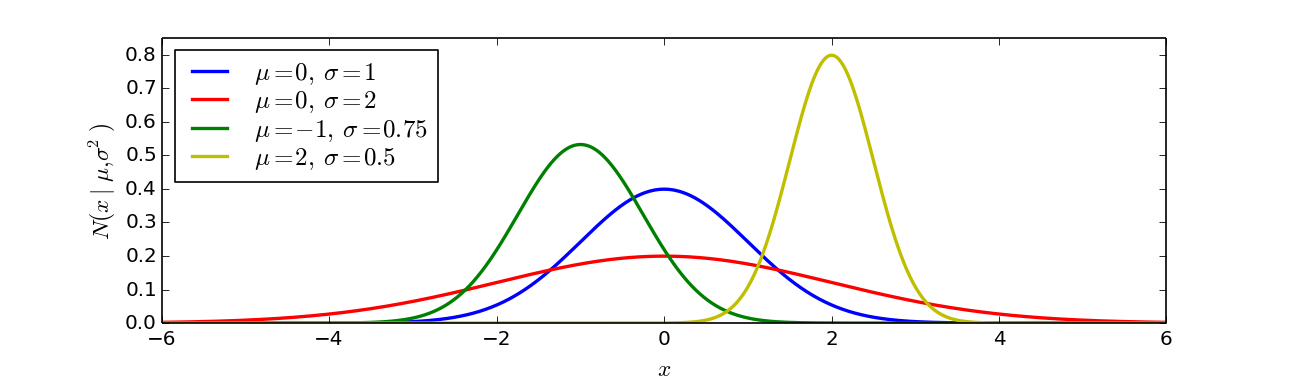
\includegraphics[width=1\textwidth]{normal.png}
    % Source: Original work by J. W. Miller.
  \end{center}
  \caption{Normal distribution with various choices of $\mu$ and $\sigma$.}
\end{figure}

The normal distribution has certain special properties that give it a unique position in probability and statistics.  Foremost among these is the central limit theorem (CLT), which states that the sum of a large number of independent random variables tends to be approximately normally distributed.  The CLT explains why real-world data so often appears approximately normal, and from a modeling perspective, it helps us to understand when a normal model would be appropriate. 

Many real-world quantities tend to be normally distributed---for instance, human heights and other body measurements, cumulative hydrologic measures such as annual rainfall or monthly river discharge, errors in astronomical or physical observations, and diffusion of a substance in a liquid or gas. Some things are products of many independent variables (rather than sums), and in such cases the logarithm will be approximately normal since it is a sum of many independent variables---this is often the case for economic quantities such as stock market indices, due to the effect of compound interest.

\subsubsection*{Basic properties of $\N(\mu,\sigma^2)$}
\begin{itemize}
\item Mean, median, and mode are all the same ($\mu$)
\item Symmetric about the mean
\item 95\% probability within $\pm 1.96\sigma$ of the mean (roughly, $\pm 2\sigma$)
\item If $X\sim\N(\mu,\sigma^2)$ and $Y\sim\N(m,s^2)$ independently, then
\begin{align}\label{equation:linear-combination}
a X + b Y\sim\N(a\mu + b m,\,a^2\sigma^2+ b^2 s^2).
\end{align}
\item Careful: \texttt{rnorm}, \texttt{dnorm}, \texttt{pnorm}, and \texttt{qnorm} in \texttt{R} take the mean and standard deviation $\sigma$ as arguments (not mean and variance $\sigma^2$). For example, \texttt{rnorm(n,m,s)} generates $n$ normal random variables from $\N(m,s^2)$.
\end{itemize}

The normal distribution is also special due to its analytic tractability---inference for complex models constructed by combining normal distributions can often be done analytically. This makes it especially convenient to work with from a computational standpoint.


% From the Bayesian perspective, the normal distribution is also special due to 


% Examples
% - Quetelet - chest sizes


\section{Conjugate prior for the mean}
\label{section:normal-normal}

Suppose we are using an i.i.d.\ normal model with mean $\theta$ and precision $\lambda$:
$$ X_1,\dotsc,X_n\iid\N(\theta,\lambda^{-1}). $$
Assume the precision $\lambda = 1/\sigma^2$ is known and fixed, and $\theta$ is given a $\N(\mu_0,\lambda_0^{-1})$ prior:
$$\btheta \sim \N(\mu_0,\lambda_0^{-1})$$
i.e., $p(\theta) = \N(\theta\mid \mu_0,\lambda_0^{-1})$. This is sometimes referred to as a \term{Normal--Normal model}.
It turns out that the posterior is
\begin{align}\label{equation:posterior}
\btheta|x_{1:n}\, \sim \,\N(M,L^{-1})
\end{align}
i.e., $p(\theta|x_{1:n}) =\N(\theta\mid M,L^{-1})$, where $L =\lambda_0+ n\lambda$ and
$$M =\frac{\lambda_0\mu_0+\lambda\sum_{i = 1}^n x_i}{\lambda_0+ n\lambda}.$$
% = \frac{n\lambda}{\lambda_0+n\lambda}\frac{1}{n}\sum_{i = 1}^n x_i +\frac{\lambda_0}{\lambda_0+ n\lambda}\mu_0.$$
Thus, the normal distribution is, itself, a conjugate prior for the mean of a normal distribution with known precision.
% todo: future: interpretation of M and L

\subsection{Derivation of the posterior}

There are various ways of deriving Equation \ref{equation:posterior}, with ``completing the square'' being perhaps the most common. Here, we take a slightly more streamlined approach. First, note that for any $x$ and $\ell$,
\begin{align}
\N(x\mid\theta,\ell^{-1})
& =\sqrt{\frac{\ell}{2\pi}}\exp\big(-\tfrac{1}{2}\ell (x-\theta)^2\big)\notag\\
&\underset{\theta}{\propto} \exp\big(-\tfrac{1}{2}\ell (x^2 - 2 x \theta +\theta^2)\big)\notag\\
&\underset{\theta}{\propto} \exp\big(\ell x \theta -\tfrac{1}{2}\ell\theta^2)\big).\label{equation:prop}
\end{align}
Due to the symmetry of the normal p.d.f.,
\begin{align}\label{equation:prior}
\N(\theta\mid\mu_0,\lambda_0^{-1}) =\N(\mu_0\mid\theta,\lambda_0^{-1})
\underset{\theta}{\propto}\exp\big(\lambda_0\mu_0\theta-\tfrac{1}{2}\lambda_0\theta^2\big)
\end{align}
by Equation \ref{equation:prop} with $x=\mu_0$ and $\ell=\lambda_0$.
Therefore, defining $L$ and $M$ as above,
\begin{align*}
p(\theta|x_{1:n})&\propto p(\theta) p(x_{1:n}|\theta) \\
&= \N(\theta\mid\mu_0,\lambda_0^{-1})\prod_{i = 1}^n\N(x_i\mid \theta,\lambda^{-1})\\
&\overset{\text{(a)}}{\propto} \exp\big(\lambda_0\mu_0\theta-\tfrac{1}{2}\lambda_0\theta^2\big)
         \exp\big(\lambda (\textstyle\sum x_i) \theta -\tfrac{1}{2}n\lambda\theta^2\big)\\
&= \exp\Big((\lambda_0\mu_0+\lambda\textstyle\sum x_i)\theta-\tfrac{1}{2}(\lambda_0+ n\lambda)\theta^2\Big)\\
&= \exp(L M\theta-\tfrac{1}{2}L\theta^2)\\
&\overset{\text{(b)}}{\propto} \N(M\mid\theta,L^{-1}) =\N(\theta\mid M,L^{-1}),
\end{align*}
where step (a) uses Equations \ref{equation:prop} and \ref{equation:prior}, and step (b) uses Equation \ref{equation:prop} with $x=M$ and $\ell=L$.


\subsection{Example: Is human height bimodal?}

The distribution of heights of adult humans---when separated according to sex (female or male)---is a classic example of a normal distribution. It seems that the reason why height tends to be normally distributed is because there are many independent genetic and environmental factors which contribute additively to overall height, and this leads to a normal distribution due to the central limit theorem. However, the combined distribution of heights (pooling females and males together) is not normal, and is often said to be bimodal---that is, having two modes (i.e., two maxima). But is it really bimodal?\footnote{This example is inspired by Schilling et al.\ (2002).}

\begin{figure}
  \begin{center}
    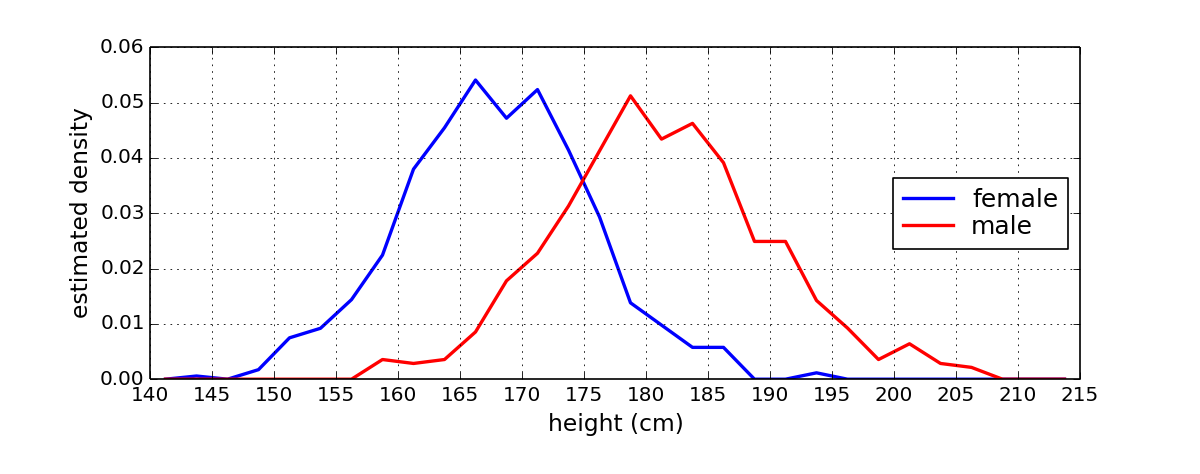
\includegraphics[width=1\textwidth]{heights-female-male.png}
    % Source: Original work by J. W. Miller.
  \end{center}
  \caption{Heights of Dutch women and Dutch men.}
  \label{figure:heights}
\end{figure}

\begin{figure}
  \begin{center}
    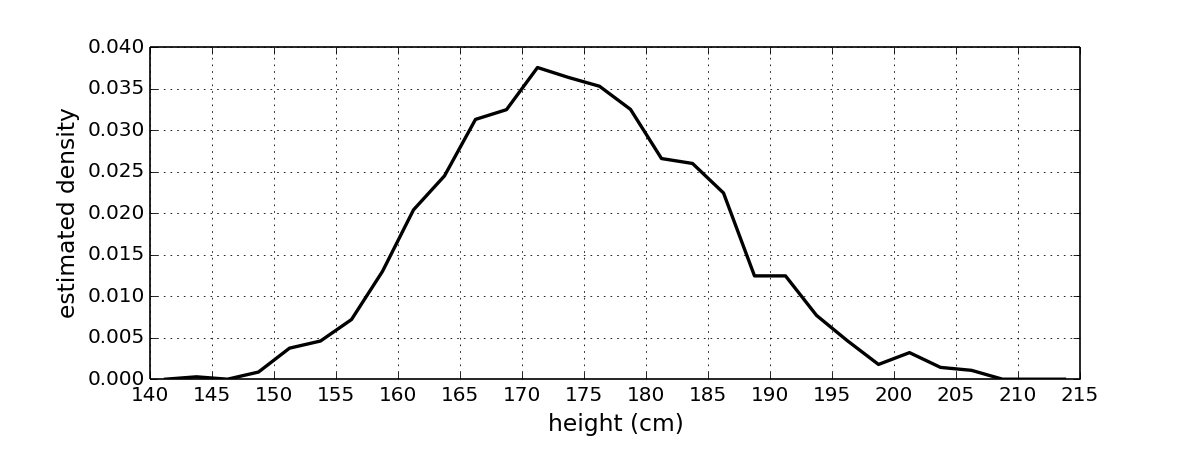
\includegraphics[width=1\textwidth]{heights-combined.png}
    % Source: Original work by J. W. Miller.
  \end{center}
  \caption{Heights of Dutch women and men, combined.}
  \label{figure:heights-combined}
\end{figure}

Figure \ref{figure:heights} shows estimated densities of the heights of Dutch women and Dutch men, based on a sample of 695 women and 562 men (Krul et al., 2011)\footnote{Data from the {\tt selfreport} dataset in the {\tt MICE} package for {\tt R}.}, and Figure \ref{figure:heights-combined} shows the estimated density for women and men together, assuming there is an equal proportion of women and men in the population.   At a glance, while the heights of women and men separately do appear to be roughly normally distributed, the combined distribution does not look bimodal.  How could we test whether it is bimodal in a more precise way?

Let's assume female heights and male heights are each normally distributed. To keep things relatively simple, let's assume they have the same standard deviation, and also that there is an equal proportion of women and men in the population. Then, it is known that the combined distribution is bimodal if and only if the difference between the means is greater than twice the standard deviation (Helguerro, 1904).

\subsubsection*{Model}

In mathematical notation: Assume the female heights are
$$X_1,\dotsc,X_k\iid\N(\theta_f,\sigma^2),$$
where $k=695$, the male heights are
$$Y_1,\dotsc,Y_\ell\iid\N(\theta_m,\sigma^2),$$
where $\ell=562$, and the p.d.f.\ of the combined distribution of heights is
$$\tfrac{1}{2}\N(x\mid\theta_f,\sigma^2)+\tfrac{1}{2}\N(x\mid\theta_m,\sigma^2). $$
(This is an example of what is called a two-component \term{mixture} distribution.) Let's put independent normal priors on $\theta_f$ and $\theta_m$:
$$ p(\theta_f,\theta_m) = p(\theta_f) p(\theta_m) 
=\N(\theta_f\mid \mu_{0,f},\sigma_0^2)\N(\theta_m\mid \mu_{0,m},\sigma_0^2).$$
In Section \ref{section:conjugate-mean-precision}, we will see how to put a prior on $\sigma^2$ (or equivalently, on $\lambda = 1/\sigma^2$), but for now, let's assume $\sigma^2$ is known.  For the purposes of this example, let's use $\sigma=8$ centimeters (about 3 inches). Based on common knowledge of typical human heights, let's choose the prior parameters (a.k.a. hyperparameters) as follows:
\begin{center}
\begin{tabular}{cll}
$\mu_{0,f}$ & (mean of prior on female mean height) & \text{165 centimeters ($\approx$ 5 feet, 5 inches)}\\
$\mu_{0,m}$ & (mean of prior on male mean height) & \text{178 centimeters ($\approx$ 5 feet, 10 inches)}\\
$\sigma_0$ & (std.\ dev.\ of priors on mean height) & \text{15 centimeters ($\approx$ 6 inches)}\\
\end{tabular}
\end{center}
Another way to choose these parameters would be to estimate them from the distribution of the mean heights in various countries around the world---and the Dutch are known for being especially tall, so that could also be taken into account. Note that $\sigma_0$ represents our uncertainty about the mean heights, not about the heights of individuals. 

It is known (Helguerro, 1904) that the combined distribution is bimodal if and only if
$$ |\theta_f-\theta_m|>2\sigma. $$
So, to address our question of interest (``Is human height bimodal?''), we would like to compute the posterior probability that this is the case, i.e., we want to know
$$ \Pr(\text{bimodal}\mid \text{data}) = \Pr\big(|\btheta_f-\btheta_m|>2\sigma \mid x_{1:k},y_{1:\ell}\big).$$
%using bold to emphasize that in this expression $\btheta_f$ and $\btheta_m$ are random variables.


\subsubsection*{Results}

\begin{figure}
  \begin{center}
    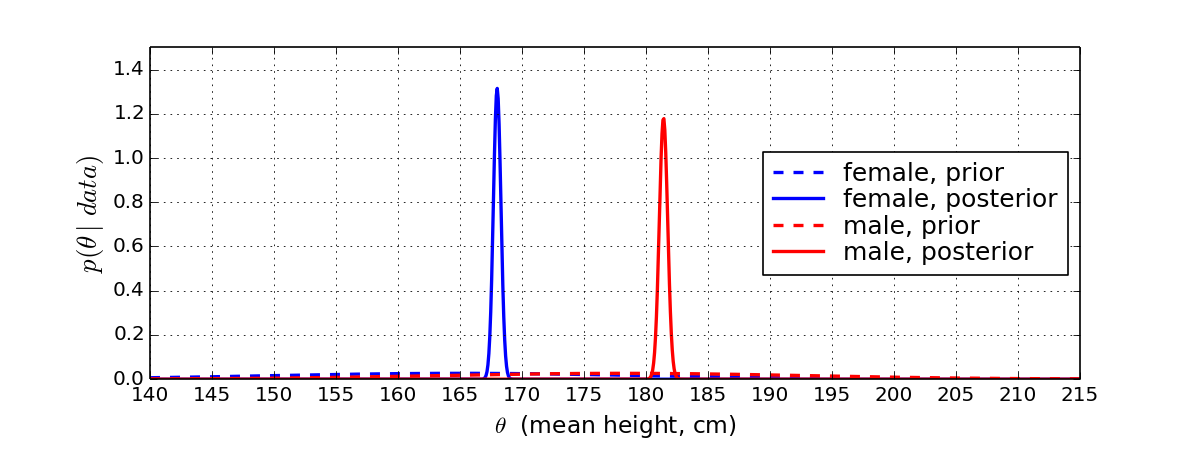
\includegraphics[width=1\textwidth]{heights-prior-posterior.png}
    % Source: Original work by J. W. Miller.
  \end{center}
  \caption{Priors and posteriors for the mean heights of Dutch women and men.}
  \label{figure:heights-prior-posterior}
\end{figure}

We can compute the posteriors for $\theta_f$ and $\theta_m$ using Equation \ref{equation:posterior} for each of them, independently.  Figure \ref{figure:heights-prior-posterior} shows the priors and posteriors. 
\begin{itemize}
\item Sample means: $\bar x = 168.0$ cm (5 feet 6.1 inches) for females, and $\bar y = 181.4$ cm (5 feet 11.4 inches) for males.
\item Posterior means: $M_f = 168.0$ cm for females, and $M_m = 181.4$ cm for males. (Essentially identical to the sample means, due to the relatively large sample size and relatively weak prior.)
\item Posterior standard deviations: $1/\sqrt{L_f} = 0.30$ cm and $1/\sqrt{L_m} = 0.34$ cm.
\end{itemize}
% The sample means are $\bar x = 168.0$ cm (5 feet 6.1 inches) for females, and $\bar y = 181.4$ cm (5 feet 11.4 inches) for males. The posterior means are nearly identical to the sample means---$M_f = 168.0$ cm for females, and $M_m = 181.4$ cm for males---due to the relatively large sample size and the relatively weak prior. The standard deviations of the posteriors are $1/\sqrt{L_f} = 0.30$ cm and $1/\sqrt{L_m} = 0.34$ cm.
By Equation \ref{equation:linear-combination} (a linear combination of independent normals is normal),
$$\btheta_m-\btheta_f\mid x_{1:k},y_{1:\ell}\,\sim\,\N(M_m-M_f,\, L_m^{-1} + L_f^{-1}) = \N(13.4,0.45^2) $$
so we can compute $\Pr(\text{bimodal}\mid \text{data})$ using the normal c.d.f.\ $\Phi$:
\begin{align*}
&\Pr(\text{bimodal}\mid \text{data})= \Pr\big(|\btheta_m-\btheta_f|>2\sigma \mid x_{1:k},y_{1:\ell}\big) \\
&= \Phi(-2\sigma\mid 13.4,0.45^2)
+ \big(1-\Phi(2\sigma\mid 13.4,0.45^2)\big)\\
& = 6.1\times 10^{-9}.
\end{align*}

Intuitive interpretation: The posteriors are about 13 or 14 centimeters apart, which is under the $2\sigma = 16$ threshold for bimodality, and they are sufficiently concentrated that the posterior probability of bimodality is essentially zero.


% Figure \ref{figure:bimodality} shows---on average---how large $\Pr(\text{bimodal}\mid \text{data})$ is when using randomly-chosen subsets of the data of increasing size. For small amounts of data, we don't know much yet about whether or not it is bimodal, but as we approach using the whole dataset of $n=k+\ell=695+562=1257$ observations, the posterior probability of bimodality decreases to near zero.

%We can compute $\lambda = 1/\sigma^2$ 






\section{Conjugate prior for the mean and precision}
\label{section:conjugate-mean-precision}

Now, suppose that both the mean $\mu$ and the precision $\lambda= 1/\sigma^2$ are unknown, with $X_1,\dotsc,X_n\iid\N(\theta,\lambda^{-1})$ as before. The $\NormalGamma(m,c,a,b)$ distribution, with $m\in\R$ and $c,a,b>0$, is a joint distribution on $(\mu,\lambda)$ obtained by letting
\begin{align*}
\bm\lambda \,\,&\sim\Ga(a,b)\\
\bm\mu|\lambda \,\,&\sim \N(m,(c\lambda)^{-1}).
\end{align*}
In other words, the joint p.d.f. is
$$ p(\mu,\lambda) = p(\mu|\lambda) p(\lambda) =\N(\mu\mid m,(c\lambda)^{-1})\Ga(\lambda\mid a,b) $$
which we will denote by $\NormalGamma(\mu,\lambda\mid m,c,a,b)$ following our usual convention.
It turns out that this provides a conjugate prior for $(\mu,\lambda)$.
Indeed, the posterior is
\begin{align}\label{equation:NormalGamma-posterior}
\bm\mu,\bm\lambda|x_{1:n}\,\sim\,\NormalGamma(M,C,A,B)
\end{align}
i.e., $p(\mu,\lambda|x_{1:n}) =\NormalGamma(\mu,\lambda\mid M,C,A,B)$, where
\begin{align*}
    M & =\frac{c m +\sum_{i=1}^n x_i}{c + n}\\
    C & = c + n\\
    A & = a + n/2\\
    B & = b +\tfrac{1}{2}\big(c m^2-C M^2+\textstyle\sum_{i=1}^n x_i^2\big).
\end{align*}
For interpretation, $B$ can also be written (by rearranging terms) as 
\begin{align}\label{equation:B}
B = b + \frac{1}{2}\sum_{i=1}^n (x_i-\bar x)^2 + \frac{1}{2}\frac{c n}{c + n}(\bar x - m)^2.
\end{align}

\subsubsection*{Interpretation of posterior parameters}
\begin{itemize}
\item $M$: Posterior mean for $\mu$. It is a weighted average (convex combination) of the prior mean and the sample mean:
$$ M =\frac{c}{c + n} m + \frac{n}{c + n}\bar x. $$
\item $C$: ``Sample size'' for estimating $\mu$. (The standard deviation of $\mu|\lambda$ is $\lambda^{-1/2}/\sqrt C$.)
\item $A$: Shape for posterior on $\lambda$. Grows linearly with sample size.
% todo: see David's notes here for degrees of freedom interpretation
\item $B$: Rate (1/scale) for posterior on $\lambda$. Equation \ref{equation:B} decomposes $B$ into the prior variation, observed variation (sample variance), and variation between the prior mean and sample mean:
$$ B = (\text{prior variation}) + \tfrac{1}{2}n\text{(observed variation)} + \tfrac{1}{2}\tfrac{c n}{c + n}\text{(variation bw means)}. $$
\end{itemize}


\subsection{Derivation of the posterior}

First, consider the NormalGamma density. Dropping constants of proportionality, multiplying out $(\mu-m)^2 =\mu^2 - 2\mu m + m^2$, and collecting terms, we have
\begin{align}
\NormalGamma(\mu,\lambda\mid m,c,a,b) &= \N(\mu\mid m,(c\lambda)^{-1})\Ga(\lambda\mid a,b)\notag\\
&= \sqrt{\frac{c\lambda}{2\pi}}\exp\Big(-\tfrac{1}{2} c\lambda(\mu-m)^2\Big)
\frac{b^a}{\Gamma(a)}\lambda^{a-1}\exp(-b\lambda)\notag\\
&\underset{\mu,\lambda}{\propto} 
\lambda^{a-1/2}\exp\Big(-\tfrac{1}{2}\lambda(c\mu^2 - 2 c m\mu + c m^2 + 2 b)\Big).\label{equation:NormalGamma}
\end{align}
Similarly, for any $x$,
\begin{align}
\N(x\mid\mu,\lambda^{-1}) & =\sqrt{\frac{\lambda}{2\pi}}\exp\Big(-\tfrac{1}{2}\lambda(x-\mu)^2\Big)\notag\\
&\underset{\mu,\lambda}{\propto} \lambda^{1/2}\exp\Big(-\tfrac{1}{2}\lambda(\mu^2 - 2 x \mu + x^2)\Big).
\label{equation:individual}
\end{align}
Using Equations \ref{equation:NormalGamma} and \ref{equation:individual}, we get
\begin{align*}
p(\mu,\lambda|x_{1:n}) &\underset{\mu,\lambda}{\propto} p(\mu,\lambda) p(x_{1:n}|\mu,\lambda) \\
& = \NormalGamma(\mu,\lambda\mid m,c,a,b) \prod_{i = 1}^n \N(x_i\mid\mu,\lambda)\\
&\underset{\mu,\lambda}{\propto}
\lambda^{a-1/2} \exp\Big(-\tfrac{1}{2}\lambda(c\mu^2 - 2 c m\mu + c m^2 + 2 b)\Big)\\
  & \qquad\times \lambda^{n/2} \exp\Big(-\tfrac{1}{2}\lambda(n\mu^2 - 2 (\textstyle\sum x_i) \mu + \sum x_i^2)\Big)\\
& = \lambda^{a+n/2-1/2}
\exp\Big(-\tfrac{1}{2}\lambda\big((c+n)\mu^2 - 2 (c m +\textstyle\sum x_i) \mu + c m^2 + 2 b + \sum x_i^2\big)\Big)\\
&\overset{\text{(a)}}{=}\lambda^{A-1/2}\exp\Big(-\tfrac{1}{2}\lambda\big(C\mu^2 - 2 C M \mu + C M^2 + 2 B\big)\Big)\\
&\overset{\text{(b)}}{\propto} \NormalGamma(\mu,\lambda\mid M,C,A,B)
\end{align*}
where step (b) is by Equation \ref{equation:NormalGamma},
and step (a) holds if $A=a+n/2$, $\,C=c+n$, $\,C M = (c m + \textstyle\sum x_i)$, and
$$C M^2 + 2 B = c m^2 + 2 b + \sum x_i^2. $$
This choice of $A$ and $C$ match the claimed form of the posterior, and 
solving for $M$ and $B$, we get $M = (c m + \sum x_i)/(c+n)$ and 
$$ B = b +\tfrac{1}{2}(c m^2-C M^2+\textstyle\sum x_i^2), $$
as claimed.



\subsection{The Pygmalion effect}
\label{section:Pygmalion}

Do a teacher's expectations influence student achievement? In a famous study, Rosenthal and Jacobson (1968) performed an experiment in a California elementary school to try to answer this question. At the beginning of the year, all students were given an IQ test.  For each class, the researchers randomly selected around 20\% of the students, and told the teacher that these students were ``spurters'' that could be expected to perform particularly well that year. (This was not based on the test---the spurters were randomly chosen.) At the end of the year, all students were given another IQ test. 
The change in IQ score for the first-grade students was:\footnote{The original data is not available. This data is from the \texttt{ex1321} dataset of the \texttt{R} package \texttt{Sleuth3}, which was constructed to match the summary statistics and conclusions of the original study.}
\begin{quote}
spurters (S)\\
$x$ = (18, 40, 15, 17, 20, 44, 38)
\end{quote}
\begin{quote}
controls (C)\\
$y$ = (--4, 0, --19, 24, 19, 10, 5, 10, 29, 13, --9, --8, 20, --1, 12, 21, --7, 14,
     13, 20, 11, 16, 15, 27, 23, 36, --33, 34, 13, 11, --19, 21, 6, 25, 30,
     22, --28, 15, 26, --1, --2, 43, 23, 22, 25, 16, 10, 29)
\end{quote}

\begin{figure}
  \begin{center}
    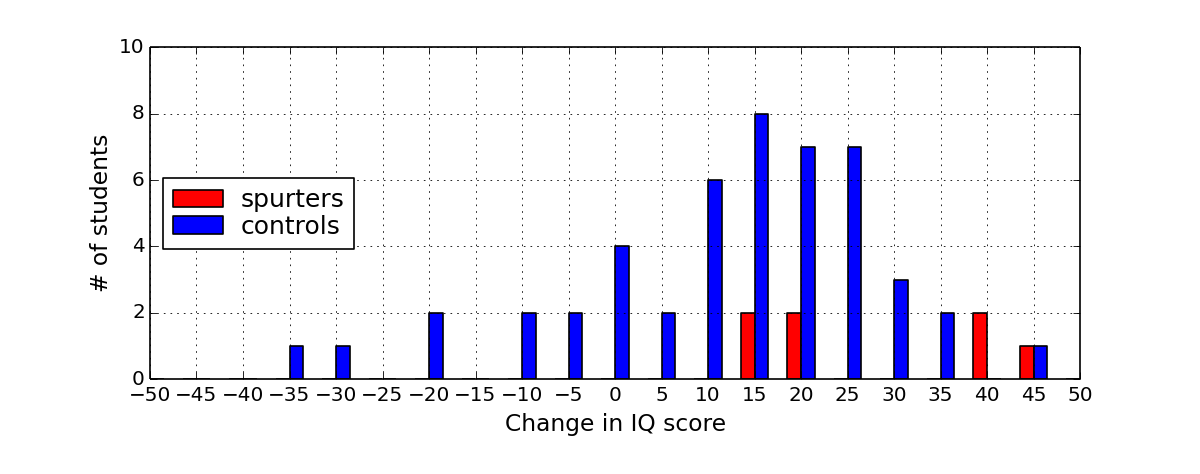
\includegraphics[width=1\textwidth]{pygmalion-histogram.png}
    % Source: Original work by J. W. Miller.
  \end{center}
  \caption{Histograms of change in IQ score for the two groups.}
  \label{figure:pygmalion-histogram}
\end{figure}
Summary statistics:
\begin{itemize}
\item spurters: $n_S = 7$, $\bar x = 27.4$, $\hat\sigma_x = 11.7$
\item controls: $n_C = 48$, $\bar y = 12.0$, $\hat\sigma_y = 16.1$
\end{itemize}
See histograms in Figure \ref{figure:pygmalion-histogram}. The average increase in IQ score is larger for the spurters.  How strongly does this data support the hypothesis that the teachers' expectations caused the spurters to perform better than their classmates? 


\subsubsection*{Model}
IQ tests are purposefully calibrated to make the scores normally distributed, so it makes sense to use a normal model here:
\begin{align*}
\text{spurters: } X_1,\dotsc,X_{n_S}\iid \N(\mu_S,\lambda_S^{-1})\\
\text{controls: } Y_1,\dotsc,Y_{n_C}\iid \N(\mu_C,\lambda_C^{-1}).
\end{align*}
We are interested in the difference between the means---in particular, is $\mu_S>\mu_C$?
We don't know the standard deviations $\sigma_S=\lambda_S^{-1/2}$ and $\sigma_C=\lambda_C^{-1/2}$, and the sample seems too small to estimate them very well.
% todo: check this claim about the frequentist approach --- I copied it from David notes
The frequentist approach to this problem is rather complicated when $\sigma_S\neq\sigma_C$ (involving approximate $t$-distributions based on the Welch--Satterthwaite degrees of freedom). 

On the other hand, it is easy using a Bayesian approach: we just need to compute the posterior probability that $\mu_S>\mu_C$:
$$ \Pr(\bm\mu_S > \bm\mu_C \mid x_{1:n_S},y_{1:n_C}). $$
Let's use independent NormalGamma priors:
\begin{align*}
\text{spurters: } (\bm\mu_S,\bm\lambda_S) \sim \NormalGamma(m,c,a,b)\\
\text{controls: } (\bm\mu_C,\bm\lambda_C) \sim \NormalGamma(m,c,a,b)
\end{align*}
with the following hyperparameter settings, based on subjective prior knowledge:
\begin{itemize}
\item $m = 0$ (Don't know whether students will improve or not, on average.)
\item $c = 1$ (Unsure about how big the mean change will be---prior certainty in our choice of $m$ assessed to be equivalent to one datapoint.)
\item $a = 1/2$ (Unsure about how big the standard deviation of the changes will be.)
\item $b = 10^2 a$ (Standard deviation of the changes expected to be around $10 = \sqrt{b/a} = \E(\lambda)^{-1/2}$.)
\end{itemize}
\begin{figure}
  \begin{center}
    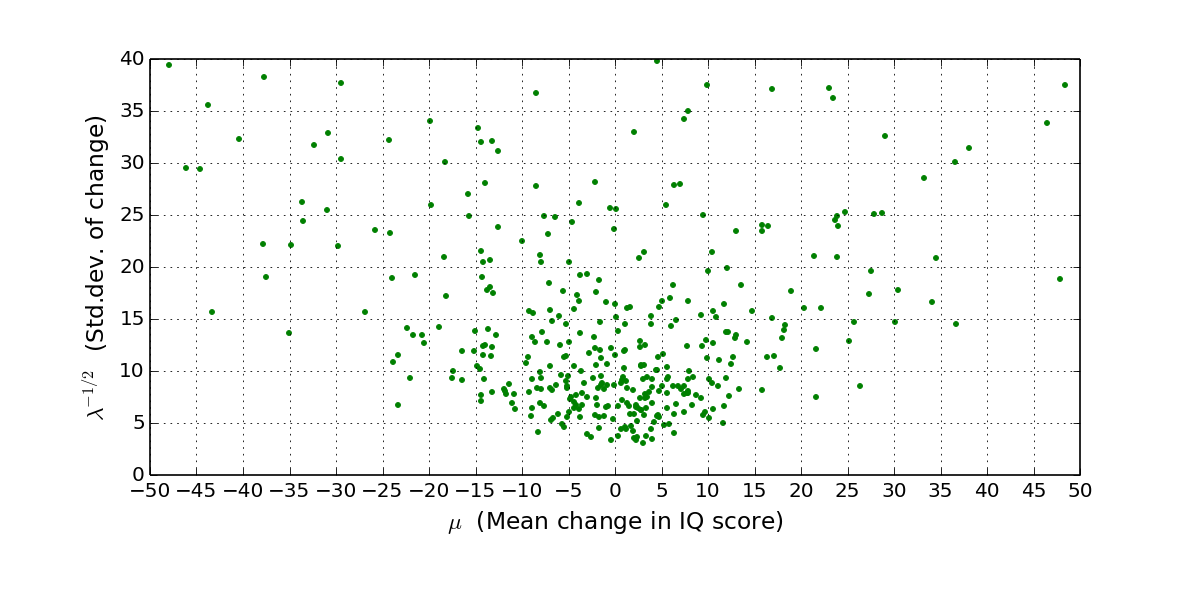
\includegraphics[width=1\textwidth]{pygmalion-prior.png}
    % Source: Original work by J. W. Miller.
  \end{center}
  \caption{Samples of $(\mu,\sigma)$ from the prior.}
  \label{figure:pygmalion-prior}
\end{figure}
Aside: How to check whether a prior conforms to our beliefs?
\begin{enumerate}
\item Draw some samples from the prior and look at them---this is probably the best general strategy. See Figure \ref{figure:pygmalion-prior}. It's also a good idea to look at sample hypothetical datasets $X_{1:n}$ drawn using these sampled parameter values. 
\item Plot the c.d.f.\ and check various quantiles (first quartile, median, third quartile), if univariate.
\item Plot the p.d.f., but beware---it can be misleading.
\item Look at various moments (e.g., mean, standard deviation), but beware---they can be misleading.
\end{enumerate}

% Note: We could instead use different values of $m,c,a,b$ for spurters and controls without any difficulty.


\subsubsection*{Results}

\begin{figure}
  \begin{center}
    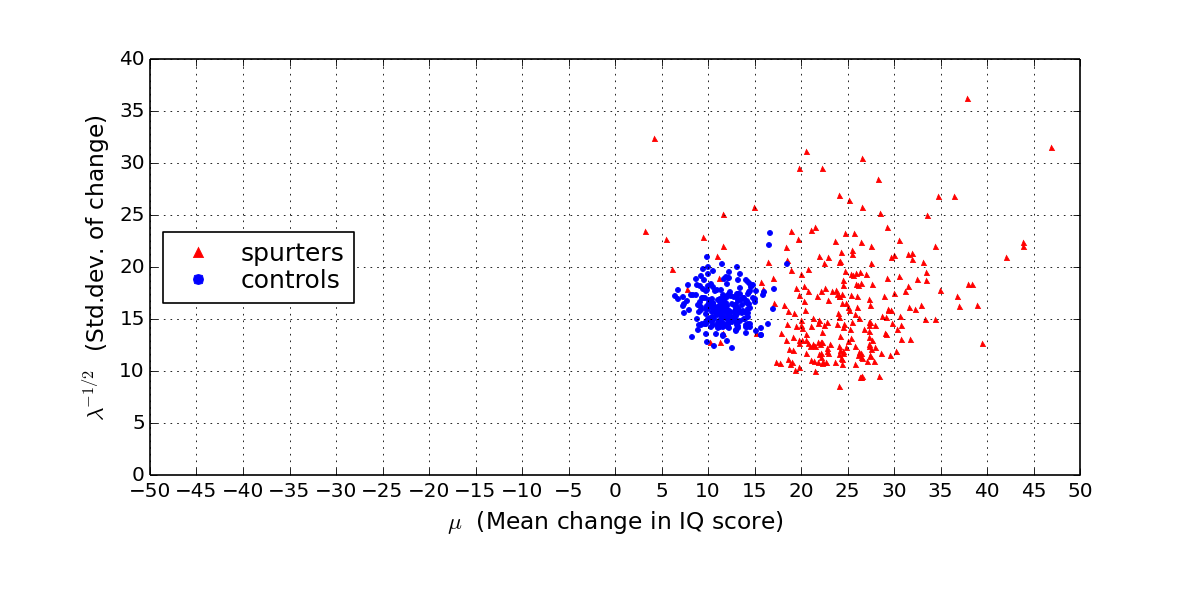
\includegraphics[width=1\textwidth]{pygmalion-posteriors.png}
    % Source: Original work by J. W. Miller.
  \end{center}
  \caption{Samples of $(\mu,\sigma)$ from the posteriors for the two groups.}
  \label{figure:pygmalion-posteriors}
\end{figure}

Using Equation \ref{equation:NormalGamma-posterior}, the posterior parameters are
\begin{align*}
\text{for spurters:} & \\
    M & =\frac{1\cdot 0 + 7 \cdot 27.43}{1 + 7} = 24.0\\
    C & = 1 + 7 = 8\\
    A & = 1/2 + 7/2 = 4\\ 
    B &= 100/2 + \tfrac{1}{2}\cdot 7\cdot 11.66^2 + \tfrac{1}{2}\frac{1\cdot 7}{1 + 7}(27.43 - 0)^2 = 855.0 \\
\text{for controls:} & \\
    M & =\frac{1\cdot 0 + 48\cdot 12.04}{1 + 48} = 11.8\\
    C & = 1 + 48 = 49\\
    A & = 1/2 + 48/2 = 24.5\\
    B &= 100/2 + \tfrac{1}{2}\cdot 48\cdot 16.10^2 + \tfrac{1}{2}\frac{1\cdot 48}{1 + 48}(12.04 - 0)^2 = 6344.0
\end{align*}
and so the posteriors are
\begin{align*}
\bm\mu_S,\bm\lambda_S\mid x_{1:n_S} &\,\sim\,\NormalGamma(24.0,8,4,855.0)\\
\bm\mu_C,\bm\lambda_C\mid y_{1:n_C} &\,\sim\,\NormalGamma(11.8,49,24.5,6344.0).
\end{align*}
Figure \ref{figure:pygmalion-posteriors} shows a scatterplot of samples from the posteriors. Now, we can answer our original question: ``What is the posterior probability that $\mu_S>\mu_C$?'' The easiest way to do this is to take a bunch of samples from each of the posteriors, and see what fraction of times we have $\mu_S>\mu_C$. This is an example of a Monte Carlo approximation (much more to come on this in the future). To do this, we draw $N=10^6$ samples from each posterior:
\begin{align*}
&(\mu_S^{(1)},\lambda_S^{(1)}),\dotsc,(\mu_S^{(N)},\lambda_S^{(N)})\sim \NormalGamma(24.0,8,4,855.0)\\
&(\mu_C^{(1)},\lambda_C^{(1)}),\dotsc,(\mu_C^{(N)},\lambda_C^{(N)})\sim\NormalGamma(11.8,49,24.5,6344.0)
\end{align*}
and obtain the approximation
\begin{align*}
\Pr(\bm\mu_S > \bm\mu_C \mid x_{1:n_S},y_{1:n_C}) 
\approx \frac{1}{N} \sum_{i = 1}^N \I\big(\mu_S^{(i)}>\mu_C^{(i)}\big) = 0.97.
\end{align*}
This is consistent with a visual inspection of the scatterplots of posteriors in Figure \ref{figure:pygmalion-posteriors}.

Interpretation: The posterior probability that the spurter group had a higher mean change in IQ score is about 0.97. Thus, this data seems to support the hypothesis that the teachers' expectations did in fact play a role. 
(Note: The results of this study have been contested, since it has been difficult to replicate.)


% \item $m = 0$ (Don't know whether students will improve or not, on average.)
% \item $c = 1$ (Unsure about how big the mean change will be---prior knowledge assessed to be equivalent to one datapoint.)
% \item $a = 1/2$ (Unsure about how big the standard deviation of the changes will be.)
% \item $b = 10^2 a$ (Standard deviation of the changes expected to be around $10 = \sqrt{b/a} =


% Summary statistics:
% n(x) = 7
% n(y) = 48
% mean(x) = 27.428571428571427
% mean(y) = 12.041666666666666
% std(x) = 11.660153672806779
% std(y) = 16.102482124056387
% posterior_x: M,C,A,B = 24.0, 8, 4.0, 855.0
% posterior_y: M,C,A,B = 11.795918367346939, 49, 24.5, 6343.979591836734

% Probability that the Pygmalion group improved more:
% P(mu_x > mu_y | data) = 0.9708023

% Probability that the standard deviation of the Pygmalion group is higher:
% P(sigma_x > sigma_y | data) = 0.415626



% todo:
% - Snowfall in Aomori vs Valdez (AK) vs Buffalo
% Show bivariate plot of prior and posterior (mu vs sigma)
% What is the probability that Aomori has more snow than Valdez, on average? (as in lab)
% What is the probability that Aomori will have more snow than Valdez in a given year? (compare posterior predictives)


% \section{Non-conjugate prior for the mean and variance}


\subsection{Inverse Gamma}

If $X$ is Gamma distributed then the distribution of $1/X$ is called the Inverse Gamma distribution. More precisely, if $X\sim\Ga(a,b)$ and $Y=1/X$ then $Y\sim \InvGamma(a,b)$, and the p.d.f.\ of $Y$ is
$$\InvGamma(y|a,b) = \frac{b^a}{\Gamma(a)} y^{-a-1}\exp(-b/y). $$
So, putting a $\Ga(a,b)$ prior on the precision $\lambda$ is equivalent to putting an $\InvGamma(a,b)$ prior on the variance $\sigma^2 = 1/\lambda$. The Inverse Gamma can be used to define a NormalInvGamma distribution for use as a prior on $(\mu,\sigma^2)$, which is sometimes more convenient than (but equivalent to) using a NormalGamma prior on $(\mu,\lambda)$.


\section{History}

In 1809, Carl Friedrich Gauss (1777--1855) proposed the normal distribution as a model for the errors made in astronomical measurements, as a formal way of justifying the use of the sample mean, by showing it to be the most likely estimate---that is, the maximum likelihood estimate---of the true value (and more generally, to justify the method of least squares in linear regression). With astonishing speed, following Gauss' proposal, Laplace proved the central limit theorem in 1810.  Laplace also calculated the normalization constant of the normal distribution, which is not a trivial task.  James Clerk Maxwell (1831--1879) showed that the normal distribution arose naturally in physics, particularly in thermodynamics.  Adolphe Quetelet (1796--1874) pioneered the use of the normal distribution in the social sciences.

\begin{figure}
    \centering
    \begin{subfigure}[t]{0.33\textwidth}
        \centering
        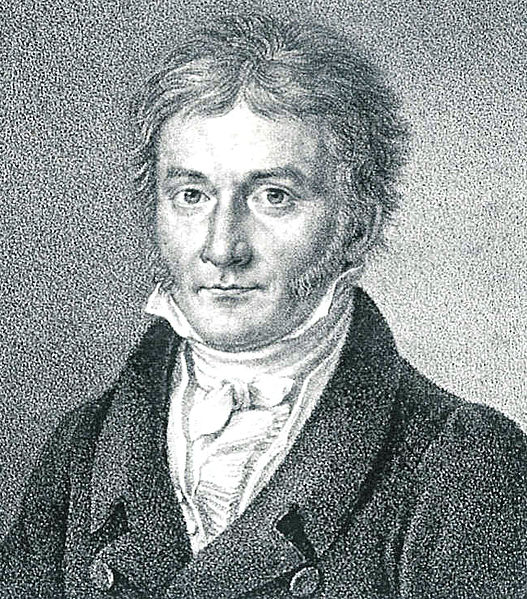
\includegraphics[height=2in]{gauss.jpg}
        % Source: http://commons.wikimedia.org/wiki/File:Bendixen_-_Carl_Friedrich_Gau%C3%9F,_1828.jpg
        % License: Public domain?
        % Date accessed: 1/25/2014
        \caption*{Carl Friedrich Gauss}
    \end{subfigure}%
    ~ 
    \begin{subfigure}[t]{0.33\textwidth}
        \centering
        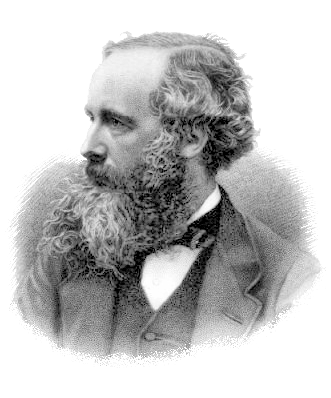
\includegraphics[trim=0 1cm 0 0, clip, height=2in]{maxwell.png}
        % Source: http://commons.wikimedia.org/wiki/File:James_Clerk_Maxwell.png
        % License: Public domain?
        % Date accessed: 1/25/2014        
        \caption*{James Clerk Maxwell}
    \end{subfigure}%
    ~
    \begin{subfigure}[t]{0.33\textwidth}
        \centering
        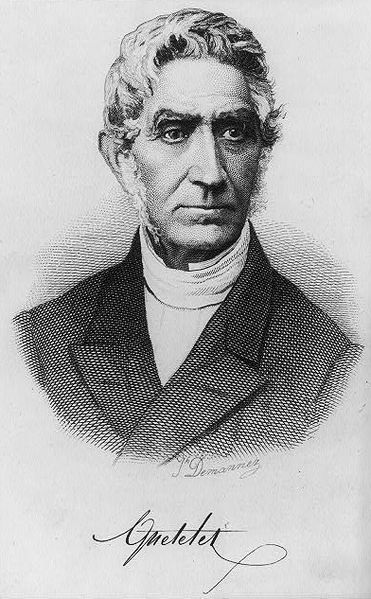
\includegraphics[trim=0 5cm 0 0, clip, height=2in]{quetelet.jpg}
        % Source: http://commons.wikimedia.org/wiki/File:Adolphe_Qu%C3%A9telet_by_Joseph-Arnold_Demannez.jpg
        % License: Public domain? 
        % Date accessed: 1/25/2014
        \caption*{Adolphe Quetelet}
    \end{subfigure}
    % \caption{Caption place holder}
\end{figure}




\newpage
\section{Exercises}

\subsubsection*{Normal--Normal model}
% In 1882, Simon Newcomb made 66 measurements of the amount of time it took for light to travel from his laboratory on the Potomac River, to a mirror placed at the base of the Washington Monument, and back. Converted to speed, in units of $\times 10^8$ meters/second, his data was as follows:

% \begin{center}
% \begin{tabular}{llllll}
% 2.9974 & 2.9976 & 2.9968 & 2.9979 & 2.9966 & 3.0061 \\ 
% 2.9975 & 2.9988 & 2.9959 & 3.0010 & 2.9973 & 2.9981 \\
% 2.9979 & 2.9982 & 2.9977 & 2.9971 & 2.9980 & 2.9973 \\
% 2.9970 & 2.9985 & 2.9979 & 2.9983 & 2.9964 & 2.9969 \\
% 2.9964 & 2.9974 & 2.9977 & 2.9982 & 2.9974 & 2.9973 \\
% 2.9963 & 2.9977 & 2.9974 & 2.9976 & 2.9971 & 2.9969 \\
% 2.9964 & 2.9976 & 2.9971 & 2.9981 & 2.9964 & 2.9980 \\
% 2.9975 & 2.9975 & 2.9974 & 2.9975 & 2.9970 & 2.9975 \\
% 2.9976 & 2.9968 & 2.9976 & 2.9969 & 2.9969 & 2.9979 \\
% 2.9960 & 2.9974 & 2.9979 & 2.9977 & 2.9969 & 2.9977 \\
% 2.9973 & 2.9975 & 2.9974 & 2.9973 & 2.9988 & 2.9980 \\
% \end{tabular}
% \end{center}
% Let $\theta$ be the speed of light, and consider a normal model for Newcomb's data:
% $$X_1,\dotsc,X_n\iid\N(\theta,\lambda^{-1}).$$
% Assume $\lambda$ is known and $\theta$ has been given a $\N(\mu_0,\lambda_0^{-1})$ prior. Suppose $\mu_0=3$ and $\lambda_0 = 1/\sigma_0^2 = 1$.

\begin{enumerate}
\item \label{exercise:predictive} Derive the posterior predictive density $p(x_{n +1}|x_{1:n})$ for the Normal--Normal model from Section \ref{section:normal-normal}. (HINT: There is an easy way to do this and a hard way. The easy way uses Equation \ref{equation:linear-combination}, writing $X_{n+1} = \btheta + Z$ given $x_{1:n}$, where $Z\sim\N(0,\lambda^{-1})$.)
\item Get a cup of hot tea or coffee and take a little break.
%\item In Newcomb's data, $x_6 = 3.0061$ appears to be an outlier.  Consider the conditional distribution of $x_6$ given the rest of the data points, that is, $p(x_6|x_{(1:n)-6})$ where $(1:n)-6$ denotes all of the indices except for $6$. Using your result from Exercise \ref{exercise:predictive}, compute the posterior predictive probability of obtaining a value at least as large as $3.0061$, that is,
% $$ \Pr(X_6>3.0061\mid x_{(1:n)-6}). $$
% On average, about how many times would you have to sample from the conditional distribution $X_6|x_{(1:n)-6}$ before seeing a value at least as large as $3.0061$?  Techniques similar to this are used for outlier detection.
% % Comparing this to our sample size indicates that something is wrong. 
\end{enumerate}

\subsubsection*{NormalGamma--Normal model}

Two competitors for the snowiest city in the world are Aomori City in Japan, and Valdez in the state of Alaska. Here are annual snowfall records, in inches/year, for the two cities: 
\begin{quote}
Aomori, 1954--2014 \\
188.6, 244.9, 255.9, 329.1, 244.5, 167.7, 298.4, 274.0, 241.3, 288.2, 208.3, 311.4, 273.2, 395.3, 353.5, 365.7, 420.5, 303.1, 183.9, 229.9, 359.1, 355.5, 294.5, 423.6, 339.8, 210.2, 318.5, 320.1, 366.5, 305.9, 434.3, 382.3, 497.2, 319.3, 398.0, 183.9, 201.6, 240.6, 209.4, 174.4, 279.5, 278.7, 301.6, 196.9, 224.0, 406.7, 300.4, 404.3, 284.3, 312.6, 203.9, 410.6, 233.1, 131.9, 167.7, 174.8, 205.1, 251.6, 299.6, 274.4, 248.0
\end{quote}
\begin{quote}
Valdez, 1976--2013 \\
351.0, 379.3, 196.1, 312.3, 301.4, 240.6, 257.6, 304.5, 296.0, 338.8, 299.9, 384.7, 353.5, 312.8, 550.7, 327.1, 515.8, 343.4, 341.6, 396.9, 267.3, 230.6, 277.4, 341.0, 377.0, 391.3, 337.0, 250.4, 353.7, 307.7, 237.5, 275.2, 271.4, 266.5, 318.7, 215.5, 438.3, 404.6
\end{quote}
% todo: record where I got this data
Assume that for each city independently, the data is i.i.d.\ normal.
\begin{enumerate}
\setcounter{enumi}{2}
\item Do you think an i.i.d.\ normal model is appropriate here? Why or why not?
\item \label{exercise:snow} Is the mean annual snowfall for Valdez higher than that of Aomori?
To address this question, perform an analysis like the one for the Pygmalion effect in Section \ref{section:Pygmalion}. In particular, your analysis should involve computing the posterior probability that the mean annual snowfall for Valdez higher than that of Aomori. Choose prior parameters (hyperparameters) according to your personal subjective prior.
\item (Continuation of Exercise \ref{exercise:snow}) Try different values for the hyperparameters, to see what effect they have on the results. Report your results for three different settings of the hyperparameters.
\end{enumerate}





\section*{Supplementary material}
\begin{itemize}
\item Hoff (2009), Chapter 5.
\item mathematicalmonk videos, Machine Learning (ML) 7.9 and 7.10 \\ 
    \url{https://www.youtube.com/playlist?list=PLD0F06AA0D2E8FFBA}
\end{itemize}

\section*{References}
\begin{itemize}
\item Schilling, M. F., Watkins, A. E., \& Watkins, W. (2002). Is human height bimodal? The American Statistician, 56(3), 223-229.
\item Krul, A. J., Daanen, H. A., \& Choi, H. (2011). Self-reported and measured weight, height and body mass index (BMI) in Italy, the Netherlands and North America. The European Journal of Public Health, 21(4), 414-419.
\item Helguerro, F. (1904), Sui Massimi Delle Curve Dimorfiche. Biometrika, 3, 85-98. 
\item Rosenthal, R., \& Jacobson, L. (1968). Pygmalion in the classroom. The Urban Review, 3(1), 16-20.
\end{itemize}




\end{document}






